\documentclass[a4paper,12pt]{article}
\usepackage[utf8]{inputenc} % Utilisation d'UTF-8 pour l'encodage des caractères
\usepackage{graphicx} % Pour inclure des images
\usepackage{amsmath} % Pour les symboles mathématiques
\usepackage{amsfonts} % Pour les polices mathématiques
\usepackage{hyperref} % Pour ajouter des liens hypertextes
\usepackage[italian]{babel} % Pour les règles de typographie en italien
\usepackage[bottom=0.5in]{geometry} % Pour ajuster les marges du document
\usepackage{bold-extra} % Pour les polices en gras supplémentaires
\usepackage{fancyhdr} % Pour personnaliser les en-têtes et pieds-de-page
\usepackage{lipsum} % Pour générer du texte fictif (utile pour des exemples)
\usepackage{setspace} % Pour gérer l'interligne

\renewcommand\seriesdefault{bx} % Pour rendre la police par défaut en gras

\pagestyle{fancy} % Utilisation du package fancyhdr pour personnaliser l'en-tête et le pied-de-page

% Personnalisation de l'en-tête et du pied-de-page
\fancyhf{} % Efface les en-têtes et pieds de page par défaut
\fancyhead[L]{Jeu de Tron - Université de Caen - Année 2024/2025} % En-tête à gauche
\fancyhead[R]{\thepage} % Numéro de page à droite
\fancyfoot[C]{\thepage} % Numéro de page au pied de page au centre

% Définir un espacement de lignes
\renewcommand{\baselinestretch}{1.5} % Interligne de 1.5 pour une meilleure lisibilité

\begin{document}
  
  {
   \setlength{\topmargin}{-3cm}
   \begin{titlepage}
     \begin{center}
    
       \centerline{
\includegraphics[height=42mm]{logo.png}}
    
       \vspace{5mm}
       {\sc {\large Universit\'e de Caen Normandie \\ Département Informatique de Caen}}
    
       \vspace{5mm}
       \centerline{\hbox to 13cm{\hrulefill}}
       \vspace{0.3cm}
       \centerline{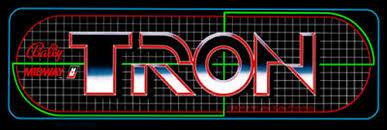
\includegraphics[height=42mm]{title.jpeg}}
       \centerline{\hbox to 13cm{\hrulefill}}
    
       \vspace{8mm}
       {\sc \large \textbf{\vspace{3mm}Réalisé par :} \\
       Medjdoub Karim \\
       Rahmoun Anes \\
       Gerouani Melissa \\
       Moudir Mohamed\\ [8mm]
       \large \textbf{\vspace{3mm}Encadré par :} \\
       Spaniol Marc \\
       François Rioult
       }
       \vspace{3mm}
    
       \hbox to \textwidth{\hrulefill}
       {\large Jeu de Tron - Année Universitaire 2024/2025}
     \end{center}
   \end{titlepage}
  }


% Table of contents page
\newpage
\tableofcontents
\newpage


\section{Introduction}
Dans le cadre de ce projet, nous avons choisi de recréer le célèbre jeu de Tron, un jeu vidéo inspiré du film de science-fiction. Ce jeu, qui se déroule dans un univers virtuel, met en scène des motos lumineuses (light cycles) qui se déplacent dans une grille. L'objectif principal est de faire en sorte que l'adversaire entre en collision avec la traînée laissée par votre moto ou avec les murs du terrain de jeu, tout en évitant de percuter votre propre ligne. Ce projet a pour but de revisiter ce classique en apportant des éléments modernes, tout en respectant l'esprit du jeu original, en termes de gameplay et de design. À travers ce projet, nous souhaitons non seulement recréer une expérience de jeu optimal mais aussi explorer des concepts de programmation, de gestion d'interactivité et d'algorithmes.

\vspace{2cm}
\begin{figure}[h]
    \centering
    
\includegraphics[height=90mm]{tron.jpeg}
    \caption{Jeu de Tron}
    \label{fig:tron}
\end{figure}

\newpage

\section{Objectifs du projet}

\subsection{Problématique}
Le projet consiste à développer une intelligence artificielle capable de jouer à Tron sans interaction humaine, en prenant des décisions stratégiques en temps réel pour éviter les collisions et maximiser sa survie. L’IA doit être compétitive et réactive dans un environnement dynamique. Le projet explore l'implémentation de l'algorithme MAXN et Paranoid pour la prise de décision multi-agent et la création d'équipes de joueurs, inspirée de l'approche SOS, afin d'optimiser la stratégie collective. Enfin, une visualisation du jeu est intégrée pour analyser les performances de chaque Algorithmes.

\subsection{Étapes principales}

\begin{enumerate}
    \item \textbf{Modélisation du jeu} :
    \begin{itemize}
        \item Définir la structure de l'environnement de jeu, incluant les éléments essentiels comme la grille (Platform) sur lequel les joueurs interagissent.
        \item Implémenter la logique des actions des joueurs, incluant les mouvements et la gestion des collisions entre les entités du jeu.
        \item Établir les règles fondamentales du jeu, telles que les conditions de déplacement des joueurs et les critères de victoire ou de défaite.
    \end{itemize}
    
    \item \textbf{Visualisation du jeu avec JavaFX} :
    \begin{itemize}
        \item Utiliser JavaFX pour créer une interface graphique pour afficher le jeu.
        \item Dessiner les joueurs, leurs traces et mettre à jour l'affichage en temps réel.
        \item Gérer l'animation des déplacements et la gestion des événements, notamment l'élimination des joueurs.
    \end{itemize}
    
    \item \textbf{Implémentation de l’IA} :
    \begin{itemize}
        \item Intégrer des algorithmes de prise de décision, notamment MAXN et Paranoid pour les joueurs contrôlés par l’IA.
        \item Définir une fonction d’évaluation basée sur des heuristiques, prenant en compte des critères tels que l’espace libre disponible, la proximité des obstacles et des adversaires.
    \end{itemize}
    
    \item \textbf{Extension pour gérer des équipes} :
    \begin{itemize}
        \item Ajouter un mécanisme de gestion des équipes dans le jeu.
        \item Adapter l’algorithme pour permettre une stratégie collective entre les membres de l’équipe.
    \end{itemize}
    
    \item \textbf{Tests et analyse des performances} :
    \begin{itemize}
        \item Lancer des simulations de parties pour observer les performances des algorthimes d'AI.
        \item Analyser l'efficacité de l’IA et ajuster les algorithmes pour améliorer les résultats.
    \end{itemize}
\end{enumerate}

\subsection{Description des travaux existants dans ce projet}

Le développement d'une IA pour jouer à Tron nécessite la mise en œuvre de plusieurs algorithmes adaptés à un environnement dynamique et compétitif. Divers travaux ont exploré des algorithmes de prise de décision dans des jeux multijoueurs, dont MAXN, Paranoid et SOS, qui ont été utilisés dans des contextes similaires.

\begin{itemize} 
    \item \textbf{MAXN} : Cet algorithme est utilisé pour gérer des jeux où plusieurs joueurs doivent prendre des décisions simultanément, en maximisant les chances de succès de chaque joueur. Il a été largement étudié dans les jeux multijoueurs où chaque agent prend en compte ses propres objectifs tout en évaluant les actions des autres joueurs. Dans les travaux existants, MAXN est souvent utilisé pour des simulations de stratégies dans des environnements complexes, notamment dans des jeux comme Tron où chaque joueur évolue sur une grille tout en cherchant à éviter les collisions.
    
    \item \textbf{Paranoid} : Similaire à MAXN, l'algorithme Paranoid prend en compte le fait que chaque joueur considère les autres joueurs comme des adversaires directs. Par conséquent, chaque joueur assume que les autres cherchent à nuire à sa propre stratégie. Cet algorithme est particulièrement utile dans des jeux multijoueurs compétitifs où les interactions entre les joueurs sont imprévisibles. Des travaux ont montré son efficacité dans la gestion de l'incertitude des actions des adversaires, en anticipant les mouvements en fonction des stratégies perçues.
    
   \item \textbf{SOS (Socially Oriented Search)} : L'algorithme SOS étend les principes de MAXN et Paranoid en introduisant des mécanismes de coopération ou d'alliance entre plusieurs joueurs. Dans des jeux où des équipes peuvent être formées, SOS permet à plusieurs joueurs de collaborer en partageant des informations et en ajustant leurs stratégies en fonction des actions des autres membres de l'équipe. Ce modèle a été utilisé dans des projets similaires où la coordination entre joueurs a un impact direct sur la performance de l’équipe.
    
    \item \textbf{Évaluation des performances} : Dans tous ces travaux, l'évaluation des performances des algorithmes est cruciale pour déterminer leur efficacité dans des environnements à grande échelle. Les évaluations incluent souvent des comparaisons entre différents algorithmes de prise de décision en fonction de paramètres tels que la taille de la grille, le nombre de joueurs, la profondeur de recherche. 
    
\end{itemize}


\newpage

\section{Fonctionnalités implémentées et leur description}

\begin{enumerate}
    \item \textbf{Déplacement des joueurs} : 
    La première fonctionnalité implémentée permet aux joueurs de se déplacer sur la plateforme tout en laissant un mur derrière eux. Contrairement à une représentation matricielle où chaque case a un contenu, notre plateforme utilise une approche où chaque joueur est représenté par une position pour sa tête et une liste de positions pour sa traînée (les positions déjà occupées par ce joueur).

    \item \textbf{Configuration du jeu via un fichier} :
    Une fonctionnalité permet de configurer les paramètres du jeu à partir d'un fichier config.txt. Ce fichier permet de sélectionner l'algorithme de prise de décision pour chaque équipe, de définir le nombre de joueurs par équipe, de spécifier la profondeur de recherche de l'IA et de déterminer la taille de la grille. Cette approche permet une personnalisation facile et flexible des paramètres du jeu sans avoir besoin de modifier le code source.

    \item \textbf{Visualisation de la configuration du jeu} :
    Une autre fonctionnalité permet d'afficher la configuration utilisée au moment du lancement du jeu dans une fenêtre dédiée. Cette fenêtre affiche les paramètres tels que l'algorithme sélectionné pour chaque équipe, le nombre de joueurs par équipe, la profondeur de recherche et la taille de la grille, offrant ainsi une vue claire et transparente de la configuration du jeu avant le début de la partie.

    \item \textbf{Modes de jeu et de benchmarking} : Le jeu propose deux modes distincts. Le premier mode permet de lancer la partie normalement avec la configuration choisie et de visualiser en temps réel les déplacements des joueurs sur la grille. Le deuxième mode, appelé "mode simulation", génère des graphiques de performance pour chaque algorithme en fonction du nombre de joueurs par équipe et de la taille de la grille, sur plusieurs parties. Ce mode permet de comparer l'efficacité des algorithmes dans diverses configurations et d'analyser leurs performances.

    \item\textbf{Visualisation avancée des états des joueurs} :
    Une fonctionnalité de visualisation avancée permet de distinguer les joueurs vivants des joueurs morts. Dès qu'un joueur meurt, sa lumière s'éteint instantanément et ses traces deviennent sombres. De plus, chaque joueur possède une couleur spécifique propre à son équipe, ce qui facilite l'identification. Le joueur survivant, ou celui ayant gagné la partie, reste le dernier à être éclairé, permettant ainsi de visualiser l'état du jeu et d'identifier rapidement le gagnant.
\end{enumerate}

\subsection{Organisation du projet}

Bien que chaque membre ait eu un rôle central dans un aspect particulier du jeu, mais dès qu'une opportunité d'amélioration ou d'ajout pertinent se présentait, tous ont contribué activement à d'autres parties du projet. chacun a apporté sa touche personnelle à tous les aspects du projet, ce qui a permis une collaboration enrichissante.

\begin{itemize}
\item \textbf{Implémentation des algorithmes et heuristiques} : Medjdoub Karim et Rahmoun Anes
\item \textbf{Visualisation graphique et interface utilisateur} : Gerouani Melissa et Medjdoub Karim
\item \textbf{Affichage du configuration , Expérimentations et analyses des performances} : Rahmoun Anes et Medjdoub Karim
\item \textbf{Gestion des déplacements et des interactions en jeu} : Moudir Mohamed et Gerouani Melissa
\item \textbf{Structure du projet et intégration du code} : Tous les membres ont contribué en améliorant et optimisant les différentes parties du projet
\item \textbf{Rédaction du rapport} : Rahmoun Anes et Moudir Mohamed
\end{itemize}


\section{Élements techniques}
\subsection{Descriptions des algorithmes}
Les trois algorithmes implémentés dans ce projet ont été développés avec des objectifs spécifiques pour l'intelligence artificielle du jeu Tron. Chacun d'eux vise à maximiser les chances de survie et la performance globale dans le jeu. Dans les sections suivantes, nous décrirons leur logique de fonctionnement ainsi que les choix d'implémentation que nous avons adoptés pour les coder:

\begin{itemize}
   \item \textbf{Maxn} :
    Cet algorithme repose sur la construction d’un arbre où chaque nœud représente un état donné du jeu dans lequel un joueur doit prendre une décision. Les branches de l’arbre correspondent aux différentes directions explorables par ce joueur. Lorsqu’un état terminal est atteint, une fonction d’évaluation, basée sur plusieurs heuristiques, attribue un vecteur de scores, où chaque composante représente le score d’un joueur. En remontant dans l’arbre, chaque joueur sélectionne le vecteur qui maximise son propre score, sans prendre en compte les décisions des autres joueurs.
    
    \item \textbf{Paranoid} :  
    Tout comme pour MAXN, nous construisons un arbre de recherche où chaque nœud représente un état donné du jeu, dans lequel un joueur doit faire un choix. Chaque branche correspond à une direction possible que le joueur peut emprunter. Lorsqu’un état terminal est atteint, une fonction d’évaluation calcule le score individuel du joueur cherchant à déterminer la meilleure direction.  

    Lors de la remontée dans l’arbre, si c'est le tour du joueur qui prend la décision, il choisit la direction qui maximise son propre score. En revanche, si c'est au tour d'un adversaire, celui-ci est considéré comme un ennemi et cherche à minimiser le score du joueur principal. Contrairement à MAXN, qui prend en compte les intérêts de tous les joueurs, Paranoid adopte une approche plus compétitive où tous les autres joueurs sont vus comme des adversaires, ce qui renforce son aspect défensif et stratégique.

    
    \item \textbf{SOS (Simultaneous Optimization Search)} :  
    Tout comme les deux premiers algorithmes, SOS construit un arbre de recherche où chaque nœud représente un état du jeu, et chaque branche correspond à une direction possible pour un joueur.  

    L’algorithme SOS agit comme un mélange entre MAXN, vis-à-vis des joueurs alliés, et Paranoid, vis-à-vis des adversaires. Lorsqu’un état terminal est atteint, une fonction d’évaluation calcule le score de l’équipe du joueur prenant la décision.  

    Lors de la remontée dans l’arbre, le joueur qui prend la décision, ainsi que ses alliés, cherchent à maximiser ce score, tandis que les adversaires tentent de le minimiser. Contrairement aux adversaires, qui sont considérés comme des ennemis, SOS suppose que les alliés agissent pour le bien de l’équipe et optimisent leurs choix en conséquence.

\end{itemize}

    \subsection{Description des données :}
1.      \textbf{Joueurs :}
        \begin{itemize}
            \item \textbf{Position de la tête} : Chaque joueur est représenté par une position correspondant à la tête de son serpent. Cette position est un couple de coordonnées $(x, y)$ où $x$ et $y$ représentent les coordonnées dans l'espace de jeu.
            \item \textbf{Liste des positions de la traînée} : En plus de la tête, chaque joueur possède une liste qui contient les positions de la traînée de son serpent. Cette liste est une collection ordonnée des positions précédentes, chaque position étant un couple de coordonnées $(x, y)$.
         \end{itemize}
   
   Exemple de structure de données :
   \begin{verbatim}
   class Bike {
       Position head; // La position de la tête (x, y)
       List<Position> Streak; // Liste des positions de la traînée
   }
   \end{verbatim}

2. \textbf{Plateforme :}
   \begin{itemize}
       \item \textbf{Ensemble des joueurs} : La plateforme est représentée par un ensemble (\texttt{Set}) contenant tous les joueurs présents. Chaque joueur est identifié de manière unique et peut être récupéré par son identifiant.
   \end{itemize}

   Exemple de structure de données :
   \begin{verbatim}
   Set<Bike> bikes; // Ensemble de joueurs présents sur la plateforme
   \end{verbatim}

   \begin{itemize}
       \item \textbf{Limites verticales et horizontales} : La plateforme a des dimensions définies par ses limites verticales et horizontales. Les indices des positions sur la plateforme sont compris entre $0$ et $taille\_plateforme$. Ainsi, la plateforme de jeu est une matrice de dimensions $taille\_plateforme \times taille\_plateforme$.
   \end{itemize}


\subsection{Paquets du projet}
Les différents paquets de ce projet sont organisés pour gérer les différentes fonctionnalités du jeu :

\begin{itemize}
    \item \textbf{View} : Ce paquet contient les classes responsables de l’affichage du jeu et de l’interface graphique.
    \begin{itemize}
        \item \texttt{GameCanvas}
        \item \texttt{GameScene}
    \end{itemize}
    
    \item \textbf{com.tronai.model} : Ce paquet définit les modèles de données utilisés dans le jeu, y compris les joueurs, les équipes, et les cellules du plateau.
    \begin{itemize}
        \item \textbf{entities} :
        \begin{itemize}
            \item \texttt{Bot}
            \item \texttt{Bike}
        \end{itemize}
        \item \textbf{platform} :
        \begin{itemize}
            \item \texttt{Direction}
            \item \texttt{Platform}
            \item \texttt{Position}
            \item \texttt{Team}
        \end{itemize}
    \end{itemize}
    
    \item \textbf{controller} : Ce paquet contient la logique de contrôle du jeu, y compris le mouvement des joueurs et la gestion de l’état du jeu.
    \begin{itemize}
        \item \texttt{Controller}
        \item \texttt{GameInitializer}
    \end{itemize}
    
    \item \textbf{Algo} : Ce paquet contient les heuristiques utilisées pour les algorithmes d’intelligence artificielle.
    \begin{itemize}
        \item \texttt{Maxn}
        \item \texttt{Minmax}
        \item \texttt{Paranoid}
    \end{itemize}
    
    \item \textbf{util} : Ce paquet contient des classes utilitaires, comme les directions et les types d’algorithmes utilisés par les équipes.
    \begin{itemize}
        \item \textbf{config} :
        \begin{itemize}
            \item \texttt{ConfigRead}
        \end{itemize}
        \item \textbf{mvc} :
        \begin{itemize}
            \item \texttt{AbstractObservable}
            \item \texttt{Observable}
            \item \texttt{Observer}
        \end{itemize}
        \item \textbf{strategie} :
        \begin{itemize}
            \item \texttt{BotStrategie}
            \item \texttt{MaxnStrategie}
            \item \texttt{ParanoidStrategie}
        \end{itemize}
    \end{itemize}
\end{itemize}

\subsection{Description des paquetages non standards utilisés}
Le projet utilise plusieurs bibliothèques non standards pour la gestion de l’interface graphique et des optimisations, notamment JavaFX et les bibliothèques pour l’algorithme Maxn et SOS.


\subsection{Description des paquetages non standards utilisés}
Le projet utilise plusieurs bibliothèques non standards pour la gestion de l’interface graphique et des optimisations, notamment JavaFX et les bibliothèques pour l’algorithme Maxn et SOS.

\newpage

\subsection{Évaluation des performances}
Les performances des algorithmes sont mesurées sur plusieurs critères :

\begin{itemize}
    \item \textbf{Nombre de mouvements} : Cela permet de déterminer l’efficacité des algorithmes en fonction de la longueur des trajets parcourus avant qu’un serpent ne soit éliminé. Des stratégies plus efficaces devraient conduire à moins de mouvements inutiles et à une gestion plus précise du terrain.
    \item \textbf{Temps d'exécution des algorithmes} : Le temps qu’un algorithme met pour prendre une décision est crucial pour le jeu en temps réel. Une IA qui met trop de temps pour calculer ses coups pourrait entraîner une expérience de jeu frustrante.
\end{itemize}

L'évaluation permet ainsi de comparer les différentes stratégies pour identifier celle qui offre le meilleur compromis entre performance et réactivité.

\newpage

\section{Fonctionnalités implémentées}

\subsection{Déplacement des motos}
Les motos sont contrôlées par l’algorithme d'IA sélectionné, qui détermine leur trajectoire en temps réel. Chaque moto évalue constamment son environnement et ajuste sa direction pour éviter les collisions tout en maximisant l'occupation de l'espace libre. La prise de décision est basée sur les informations actuelles du terrain et des adversaires.

\subsection{Stratégies d'IA}
L'IA utilise plusieurs stratégies pour interagir avec le terrain et les autres joueurs. Ces stratégies sont dynamiques et prennent en compte les changements du jeu à chaque instant. Elles permettent aux motos de répondre aux situations en temps réel.

\begin{itemize}
    \item \textbf{Maxn} : L'algorithme Maxn cherche à maximiser les chances de survie et d'expansion de la moto, tout en tenant compte des actions prévisibles des autres joueurs. Il analyse les décisions possibles de tous les joueurs et choisit celle qui offre les meilleures chances de succès.
    \item \textbf{Paranoid} : Cette stratégie met l'accent sur la défense. La moto utilisant Paranoid évite les zones risquées en anticipant les mouvements des autres motos, en cherchant à minimiser les dangers immédiats, tout en maximisant ses chances de survie.
    \item \textbf{SOS (Simultaneous Optimization Search)} : SOS coordonne les actions des motos en prenant en compte les mouvements des adversaires, cherchant à optimiser les stratégies collectives. Elle permet une gestion simultanée de plusieurs motos pour tirer parti de l'intéraction entre elles.
\end{itemize}

\subsection{Affichage du jeu}
Le jeu est rendu visuellement grâce à JavaFX, offrant une interface graphique fluide et réactive. Le terrain de jeu est mis à jour à chaque étape du jeu, affichant les déplacements des motos et leurs traces sur le plateau. Les animations des déplacements et des événements sont gérées en temps réel, créant une expérience visuelle immersive pour l'utilisateur.

\subsection{Gestion des collisions}
Les collisions avec les murs, les autres motos ou soi-même entraînent l’élimination immédiate de la moto concernée. Ce mécanisme de gestion des collisions permet de garantir une dynamique de jeu rapide et fluide, et de maintenir une expérience de jeu compétitive. La partie se termine lorsqu’un seul joueur (moto) reste en vie.

\subsection{Interface de configuration}
L'interface de configuration permet aux joueurs de personnaliser les paramètres du jeu avant le lancement. Les paramètres, tels que la taille du terrain, le nombre de joueurs (humains et IA), et les stratégies utilisées pour chaque moto, peuvent être définis à travers un fichier de propriétés. Cela permet de lancer une partie avec des configurations variées et d’adapter les règles à différentes préférences.

\subsection{Fin de partie et résultats}
La partie se termine lorsqu'une seule moto survit. Un message de victoire s'affiche à la fin de chaque partie, indiquant la moto gagnante. Après cela, les joueurs peuvent choisir de recommencer une nouvelle partie avec les mêmes ou de nouveaux paramètres. Un système de scoring ou de classement peut être intégré pour ajouter un aspect compétitif à long terme.
\newpage


\newpage

\section{Expérimentations}

\subsection{Tests d’optimisation}
Plusieurs expérimentations ont été réalisées pour tester l’efficacité des différents algorithmes (Maxn, Paranoid, et SOS) en termes de performance, de réactivité et de nombre de mouvements effectués. Ces tests ont permis d’évaluer la qualité des décisions prises par l’IA dans différentes configurations.

\subsection{Analyse des résultats}
Les résultats montrent une différence notable dans la performance des algorithmes, notamment en fonction de la complexité de l’environnement et des choix des adversaires. Les tests ont permis d’identifier les points forts et les faiblesses de chaque algorithme.

\subsection{Pistes d’amélioration}
Pour améliorer les performances de l’IA, plusieurs pistes ont été explorées :
\begin{itemize}
    \item Optimisation de l’algorithme Maxn pour mieux anticiper les mouvements des adversaires.
    \item Ajout de stratégies adaptatives pour l’IA en fonction des mouvements des autres joueurs.
    \item Amélioration de l’interface graphique pour rendre l’expérience de jeu plus immersive.
\end{itemize}

\newpage

\section{Conclusion}
Le projet a permis de développer une version interactive et compétitive du jeu Tron, avec une intelligence artificielle réactive et évolutive. Les différents algorithmes implémentés (Maxn, Paranoid et SOS) ont permis de tester différentes approches de la stratégie de jeu, chacune ayant ses avantages et ses inconvénients.

Des améliorations sont envisageables, notamment dans l’optimisation des algorithmes et la gestion de l’interface graphique, pour rendre l’expérience encore plus fluide et réaliste.

\end{document}
